\documentclass[10pt,a4paper]{article}

\usepackage[margin=2.0cm,includeheadfoot]{geometry}
\usepackage[T1]{fontenc}
\usepackage[utf8]{inputenc}
\usepackage{lmodern}
\usepackage{microtype}
\usepackage{booktabs}
\usepackage{longtable}
\usepackage{array}
\usepackage{graphicx}
\usepackage{xcolor}
\usepackage{tikz}
\usetikzlibrary{arrows.meta,positioning,fit,calc}
\usepackage{hyperref}
\usepackage{enumitem}
\usepackage{fancyhdr}
\usepackage{titlesec}

\definecolor{navy}{HTML}{17324D}
\definecolor{blue}{HTML}{236B8E}
\definecolor{teal}{HTML}{2A9D8F}
\definecolor{orange}{HTML}{E76F51}
\definecolor{lightblue}{HTML}{EAF3F7}
\definecolor{lightgreen}{HTML}{EAF6F3}
\definecolor{lightorange}{HTML}{FDF0EB}
\definecolor{ink}{HTML}{263746}

\hypersetup{colorlinks=true,linkcolor=blue,urlcolor=blue,citecolor=blue}
\urlstyle{same}
\setlength{\parindent}{0pt}
\setlength{\parskip}{5pt}
\setlist{itemsep=2pt,topsep=3pt,leftmargin=1.25em}
\renewcommand{\arraystretch}{1.18}
\color{ink}

\titleformat{\section}{\Large\bfseries\color{navy}}{\thesection.}{0.55em}{}
\titleformat{\subsection}{\normalsize\bfseries\color{blue}}{\thesubsection}{0.55em}{}
\titlespacing*{\section}{0pt}{15pt}{5pt}
\titlespacing*{\subsection}{0pt}{9pt}{2pt}

\pagestyle{fancy}
\fancyhf{}
\lhead{\color{navy}\small MLOps GBFS Bike-Sharing}
\rhead{\color{blue}\small Perancangan Arsitektur Data}
\cfoot{\color{blue}\small\thepage}
\renewcommand{\headrulewidth}{0.4pt}
\renewcommand{\headrule}{\hbox to\headwidth{\color{blue}\leaders\hrule height \headrulewidth\hfill}}

\newcommand{\code}[1]{\texttt{#1}}

\begin{document}

\begin{titlepage}
\thispagestyle{empty}
\vspace*{1.2cm}
{\color{navy}\rule{\textwidth}{3pt}}\\[1.2cm]
{\color{navy}\Huge\bfseries Dokumen Perancangan\\[0.15cm]
Arsitektur Data}\par
\vspace{0.45cm}
{\color{blue}\Large MLOps GBFS Bike-Sharing Forecasting}\par
\vspace{1.4cm}
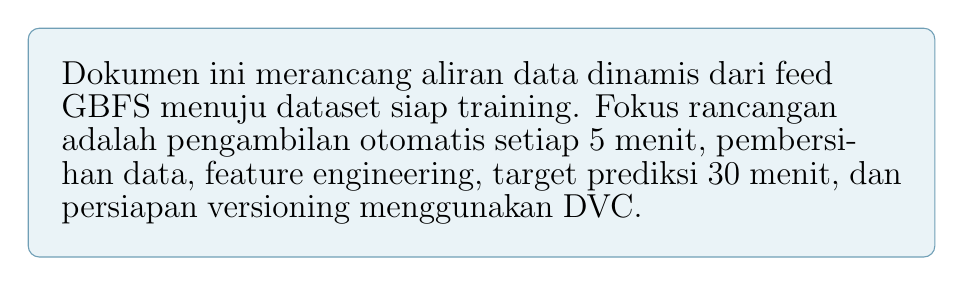
\begin{tikzpicture}
  \node[draw=blue!65, fill=lightblue, rounded corners=4pt,
        text width=0.88\textwidth, inner sep=12pt, align=left] {\large
    Dokumen ini merancang aliran data dinamis dari feed GBFS menuju dataset
    siap training. Fokus rancangan adalah pengambilan otomatis setiap 5 menit,
    pembersihan data, feature engineering, target prediksi 30 menit, dan
    persiapan versioning menggunakan DVC.};
\end{tikzpicture}
\vfill
\begin{tabular}{@{}ll@{}}
\textbf{Proyek} & MLOps GBFS Bike-Sharing Forecasting\\
\textbf{Repository} & GitHub Codespaces, struktur LK-02\\
\textbf{Luaran} & Panduan implementasi ingestion dan preprocessing LK-04\\
\textbf{Tanggal} & 21 September 2026
\end{tabular}
\vspace{0.7cm}
\par{\color{navy}\rule{\textwidth}{1.5pt}}
\end{titlepage}

\section*{Ringkasan eksekutif}
Sistem mengambil status Citi Bike melalui GBFS discovery endpoint. Setiap
polling menghasilkan satu snapshot yang berisi banyak baris stasiun dan
disimpan sebagai JSON mentah. Snapshot kemudian divalidasi, digabung dengan
informasi stasiun, diubah menjadi fitur deret waktu, dan dimuat ke dataset
siap training. Waktu $t$ dipakai untuk memprediksi kondisi pada $t+30$ menit.

\begin{center}
\begin{tabular}{>{\bfseries}p{0.25\textwidth} p{0.64\textwidth}}
\toprule
Keputusan & Rancangan \\
\midrule
Sumber & Citi Bike GBFS v2.3 melalui discovery endpoint \\
Frekuensi & Polling setiap 5 menit (300 detik) \\
Target & \code{num\_bikes\_available} dan \code{num\_docks\_available} pada $t+30$ menit \\
Unit prediksi & Satu stasiun per timestamp \\
Penyimpanan & \code{data/raw} $\rightarrow$ \code{data/interim} $\rightarrow$ \code{data/processed} \\
Versioning & Manifest hash saat ini; DVC per partisi harian pada tahap berikutnya \\
\bottomrule
\end{tabular}
\end{center}

\section{Tujuan dan ruang lingkup}
Sistem dirancang untuk membantu operator mengantisipasi stasiun yang akan
kehabisan sepeda atau slot dok. Rancangan ini mencakup perolehan data,
validasi, pembersihan, transformasi fitur, penyimpanan, dan versioning. Model
forecasting dan service inference berada di luar ruang lingkup dokumen ini.

\section{Sumber data dinamis (LK-01)}
Sumber utama adalah feed publik Citi Bike yang mengikuti General Bikeshare
Feed Specification (GBFS) v2.3. Pipeline selalu membaca discovery endpoint
berikut agar URL feed aktual diambil dari publisher:
\begin{center}
\fcolorbox{blue!45}{lightblue}{\parbox{0.88\textwidth}{\centering
\url{https://gbfs.citibikenyc.com/gbfs/2.3/gbfs.json}}}
\end{center}

\begin{longtable}{@{}p{0.28\textwidth}p{0.62\textwidth}@{}}
\toprule
\textbf{Feed} & \textbf{Peran} \\
\midrule
\code{station\_information} & Identitas stasiun, nama, koordinat, kapasitas, dan atribut lokasi. \\
\code{station\_status} & Jumlah sepeda dan slot dok tersedia, status instalasi, penyewaan, pengembalian, serta waktu laporan terakhir. \\
\bottomrule
\end{longtable}

Feed diambil setiap 5 menit. Satu polling menghasilkan satu snapshot yang
memuat banyak baris, yaitu satu baris untuk setiap stasiun yang tersedia.
Jadi, interval 5 menit adalah interval antar-snapshot untuk stasiun yang
berhasil diambil, bukan interval antarbaris di dalam satu respons.

\section{Skema data awal}
Struktur JSON mengikuti objek tingkat atas \code{version},
\code{last\_updated}, \code{ttl}, dan \code{data.stations}. Kolom inti yang
digunakan pipeline adalah:

\begin{longtable}{@{}p{0.31\textwidth}p{0.19\textwidth}p{0.38\textwidth}@{}}
\toprule
\textbf{Kolom} & \textbf{Sumber} & \textbf{Kegunaan} \\
\midrule
\code{station\_id} & Keduanya & Kunci penggabungan dan unit prediksi. \\
\code{collected\_at} & Pipeline & Waktu UTC saat request berhasil. \\
\code{last\_reported} & Status & Umur observasi dari operator. \\
\code{num\_bikes\_available} & Status & Target jumlah sepeda. \\
\code{num\_docks\_available} & Status & Target jumlah slot dok. \\
\code{capacity} & Information & Kapasitas stasiun. \\
\code{lat}, \code{lon} & Information & Posisi stasiun. \\
\code{is\_installed}, \code{is\_renting}, \code{is\_returning} & Status & Validasi dan fitur operasional. \\
\bottomrule
\end{longtable}

\section{Visualisasi arsitektur pipeline}
Gambar~\ref{fig:architecture} menunjukkan aliran data dari sumber eksternal
hingga artefak siap pakai. Kotak berwarna biru adalah komponen proses, kotak
hijau adalah lokasi data di repository, dan kotak oranye adalah keluaran
operasional atau penyimpanan versioned.

\begin{figure}[htbp]
\centering
\resizebox{\textwidth}{!}{%
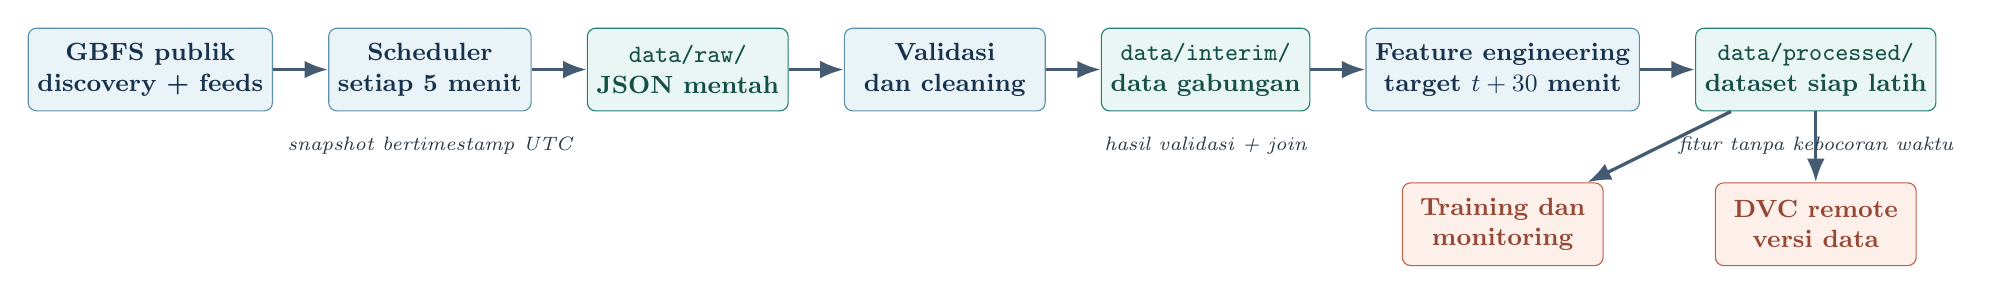
\begin{tikzpicture}[
  process/.style={draw=blue!75, fill=lightblue, rounded corners=3pt,
    minimum width=2.55cm, minimum height=1.05cm, align=center,
    font=\small\bfseries, text=navy},
  store/.style={draw=teal!80!black, fill=lightgreen, rounded corners=3pt,
    minimum width=2.55cm, minimum height=1.05cm, align=center,
    font=\small\bfseries, text=teal!50!black},
  output/.style={draw=orange!85!black, fill=lightorange, rounded corners=3pt,
    minimum width=2.55cm, minimum height=1.05cm, align=center,
    font=\small\bfseries, text=orange!65!black},
  arrow/.style={-{Latex[length=3mm]}, very thick, draw=navy!80},
  note/.style={font=\scriptsize\itshape, text=ink}
]
\node[process] (source) {GBFS publik\\discovery + feeds};
\node[process, right=7mm of source] (schedule) {Scheduler\\setiap 5 menit};
\node[store, right=7mm of schedule] (raw) {\code{data/raw/}\\JSON mentah};
\node[process, right=7mm of raw] (clean) {Validasi\\dan cleaning};
\node[store, right=7mm of clean] (interim) {\code{data/interim/}\\data gabungan};
\node[process, right=7mm of interim] (feature) {Feature engineering\\target $t+30$ menit};
\node[store, right=7mm of feature] (processed) {\code{data/processed/}\\dataset siap latih};
\node[output, below=9mm of processed] (dvc) {DVC remote\\versi data};
\node[output, below=9mm of feature] (train) {Training dan\\monitoring};
\draw[arrow] (source) -- (schedule);
\draw[arrow] (schedule) -- (raw);
\draw[arrow] (raw) -- (clean);
\draw[arrow] (clean) -- (interim);
\draw[arrow] (interim) -- (feature);
\draw[arrow] (feature) -- (processed);
\draw[arrow] (processed) -- (dvc);
\draw[arrow] (processed) -- (train);
\node[note, below=2mm of schedule] {snapshot bertimestamp UTC};
\node[note, below=2mm of interim] {hasil validasi + join};
\node[note, below=2mm of processed] {fitur tanpa kebocoran waktu};
\end{tikzpicture}}
\caption{Arsitektur aliran data untuk ingestion, ETL, dan persiapan training.}
\label{fig:architecture}
\end{figure}

\section{Rancangan pipeline ETL}
\subsection{Extract / ingestion}
Modul \code{src/data/ingest\_gbfs.py} melakukan langkah berikut:
\begin{enumerate}
  \item meminta discovery endpoint;
  \item mengambil URL \code{station\_information} dan \code{station\_status};
  \item mengirim HTTP GET dengan timeout 20 detik dan maksimal tiga percobaan;
  \item menyimpan JSON mentah dengan timestamp UTC pada \code{data/raw/};
  \item mencatat status HTTP, ukuran file, jumlah baris, field contoh, dan SHA-256 pada manifest bukti.
\end{enumerate}
Penjadwalan produksi dapat menggunakan GitHub Actions dengan cron setiap 5
menit. Karena eksekusi job dapat bergeser dan workspace job bersifat
sementara, data historis harus dikirim ke penyimpanan persisten pada tahap
implementasi DVC.

\subsection{Transform / cleaning}
Tahap pembersihan memvalidasi JSON dan memastikan field wajib tersedia.
Selanjutnya pipeline:
\begin{itemize}
  \item mengubah timestamp POSIX menjadi waktu UTC;
  \item memastikan kolom hitungan non-negatif dan kapasitas positif;
  \item menghapus duplikat berdasarkan \code{station\_id} dan waktu pengambilan;
  \item memeriksa kecocokan station ID antara dua feed;
  \item menandai observasi yang terlambat atau tidak konsisten, lalu menyimpan alasan penolakannya;
  \item menggabungkan kedua feed dengan kunci \code{station\_id}.
\end{itemize}
Hasil antara disimpan pada \code{data/interim/}. Data yang hilang tidak
langsung diisi dengan nol karena nol memiliki arti operasional yang berbeda
dari data yang tidak tersedia.

\subsection{Transform / feature engineering}
Data diurutkan per stasiun dan waktu pengambilan. Fitur awal yang direncanakan:
\begin{itemize}
  \item jam, hari dalam minggu, dan indikator akhir pekan;
  \item rasio sepeda tersedia terhadap kapasitas dan rasio slot kosong terhadap kapasitas;
  \item nilai lag 5, 10, 15, dan 30 menit;
  \item perubahan jumlah sepeda dan slot sejak observasi sebelumnya;
  \item rolling mean dan rolling standard deviation pada jendela historis.
\end{itemize}
Baris target dibuat dengan menggeser nilai masa depan sekitar enam snapshot
untuk horizon 30 menit. Fitur hanya memakai data hingga waktu $t$ agar tidak
terjadi kebocoran data. Dataset siap latih disimpan di \code{data/processed/}.

\section{Struktur repository dan aliran penyimpanan}
\begin{longtable}{@{}p{0.30\textwidth}p{0.60\textwidth}@{}}
\toprule
\textbf{Lokasi} & \textbf{Isi} \\
\midrule
\code{data/raw/} & JSON asli per snapshot; tidak diproses ulang. \\
\code{data/interim/} & Data gabungan dan hasil validasi sementara. \\
\code{data/processed/} & Dataset fitur dan target yang siap training. \\
\code{reports/evidence/} & Manifest capture yang dapat diperiksa dosen. \\
\code{config/base.yaml} & Endpoint discovery, interval 300 detik, zona waktu UTC, dan horizon 30 menit. \\
\bottomrule
\end{longtable}

\section{Rencana versioning data}
Setiap snapshot memiliki ID berdasarkan waktu UTC, misalnya
\code{20260921T120000Z}. Manifest menyimpan URL, versi GBFS, waktu capture,
\code{last\_updated}, jumlah record, ukuran file, dan hash SHA-256. Pada pekan
berikutnya, direktori data mentah dan hasil proses akan dilacak memakai DVC
per partisi harian. File metadata \code{.dvc}, \code{dvc.yaml}, dan
\code{dvc.lock} disimpan di Git; isi dataset dan cache disimpan di remote DVC.
Satu commit Git akan menjadi referensi terhadap versi kode, parameter, dan
pointer data yang dipakai untuk eksperimen.

\section{Bukti pengambilan data}
Capture aktual disimpan pada \code{reports/evidence/gbfs\_capture.json}.
Berkas tersebut dihasilkan oleh modul ingestion dan mencatat status HTTP,
versi feed, jumlah stasiun, field contoh, ukuran, serta hash setiap file mentah.

\begin{center}
\fcolorbox{teal!65!black}{lightgreen}{\parbox{0.91\textwidth}{
\textbf{Capture aktual (UTC):} 2026-09-21T15:20:57Z\\
Discovery: HTTP 200, GBFS version 2.3, TTL 60 detik\\
\code{station\_information}: HTTP 200, 2.520 record\\
\code{station\_status}: HTTP 200, 2.520 record\\
Manifest: \code{reports/evidence/gbfs\_capture.json}}}
\end{center}

\section{Kriteria penerimaan untuk LK-04}
Implementasi berikutnya dianggap sesuai rancangan apabila dapat mengunduh
kedua feed secara otomatis, menghasilkan file mentah bertimestamp, menolak
respons tidak valid dengan pesan yang jelas, menghasilkan tabel interim dan
processed tanpa kebocoran waktu, serta menulis manifest yang cukup untuk
mereproduksi satu snapshot.

\section*{Referensi}
\begin{itemize}
  \item MobilityData, \emph{General Bikeshare Feed Specification v2.3},
  \url{https://github.com/MobilityData/gbfs/blob/v2.3/gbfs.md}.
  \item Citi Bike, GBFS discovery endpoint,
  \url{https://gbfs.citibikenyc.com/gbfs/2.3/gbfs.json}.
  \item DVC, \emph{Command Reference},
  \url{https://dvc.org/doc/command-reference/}.
\end{itemize}

\end{document}
